
\subsection{Implementation}
\begin{frame}
\frametitle{Implementation}
\begin{itemize}
    \item A data type for functions real analytic on $[0,1]$ was implemented in \irram .
    \item Constructor from a single power series.
    \item Analytic continuation used if more series are needed to cover the interval. 
    \item The running time and memory usage was empirically analyzed.
    \item Running time increases quickly with number of analytic continuations. 
\end{itemize}
\end{frame}
\begin{frame}
  \frametitle{Evaluation\dots}
  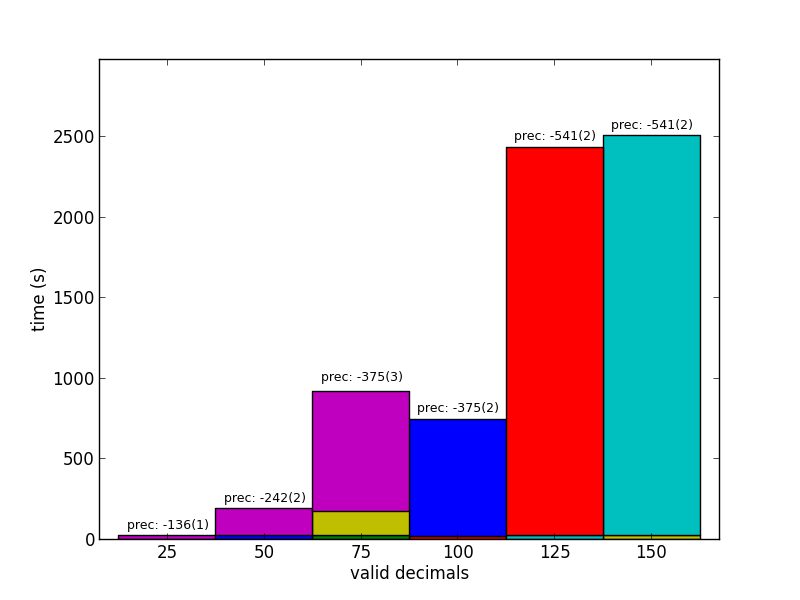
\includegraphics[width=0.9\textwidth]{sin_for_series_4_dep_on_n}
\end{frame}
\begin{frame}
  \frametitle{Evaluation\dots}
  \begin{minipage}{0.48\textwidth}
  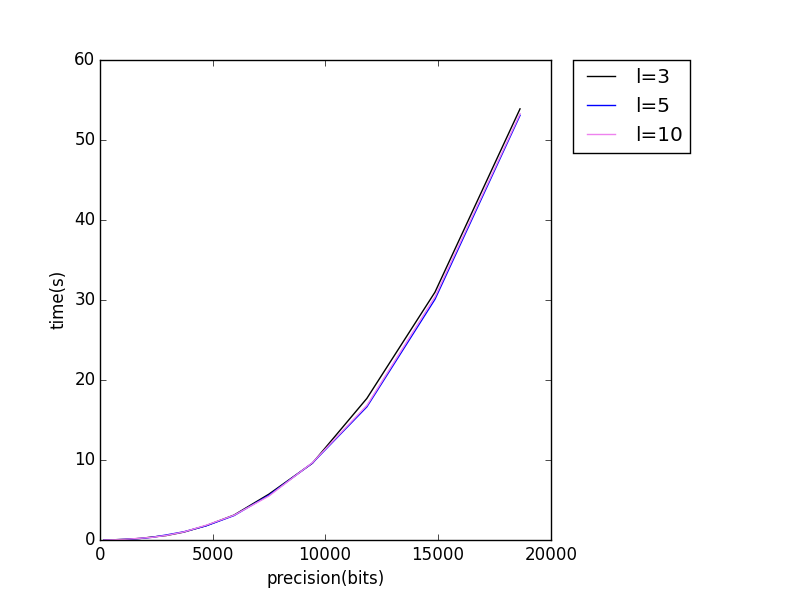
\includegraphics[width=1.2\textwidth]{time_0}
  \end{minipage}
  \begin{minipage}{0.48\textwidth}
  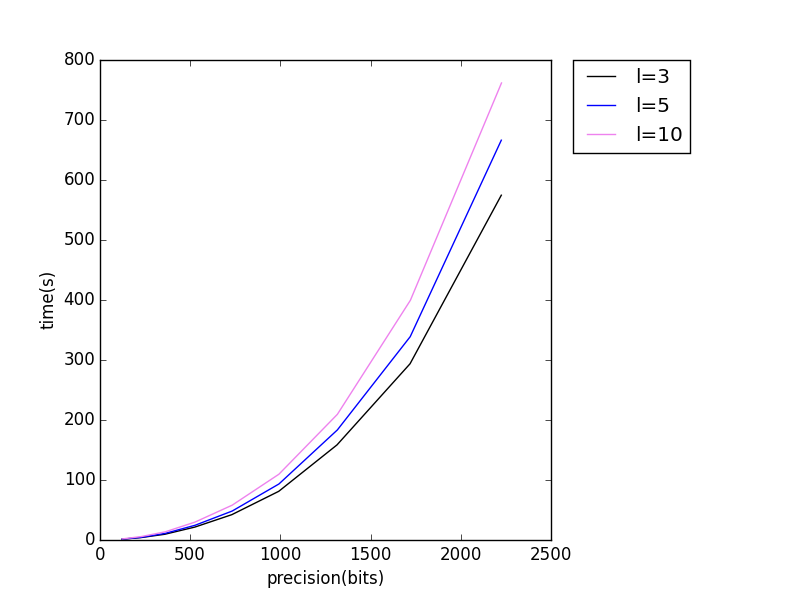
\includegraphics[width=1.2\textwidth]{time_1}
  \end{minipage}
\end{frame}
\begin{frame}
  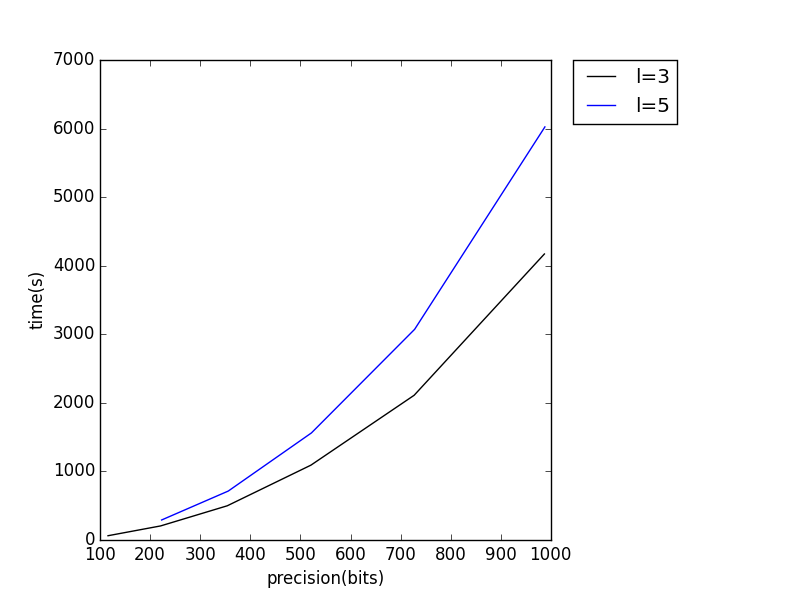
\includegraphics[width=0.8\textwidth]{time_2}
\end{frame}
\begin{frame}[t]{Riemann Mapping Theorem}
  \begin{theorem}[Riemann]
    Let $U \subsetneq \C$ be non empty, simply connected and open.
    Then there exists a biholomorphic mapping from $U$ on to the open unit disc.
  \end{theorem}
  \pause
  In the general case $\#P$ hard. (Binder, Braverman, Yampolsky)\\
  Riemann mappings of domains with polynomial time computable analytic boundaries are polynomial time computable. (Rettinger)
\end{frame}
